\documentclass[parskip=full,11pt,openany]{scrreprt}

\usepackage[sfdefault,light]{roboto}
\usepackage{inconsolata}
\usepackage[ngerman]{babel}

\usepackage[utf8]{inputenc}
\usepackage[T1]{fontenc}

\usepackage{microtype}

\usepackage{csquotes}
\MakeOuterQuote{"}

\usepackage{graphicx}
\usepackage{float}
\usepackage{bm}
\usepackage{amssymb}
\usepackage[hidelinks]{hyperref}
\usepackage[section]{placeins}
\usepackage{booktabs}

\usepackage{amsmath}

\usepackage{enumitem} 

\usepackage{amssymb}% http://ctan.org/pkg/amssymb
\usepackage{pifont}% http://ctan.org/pkg/pifont
\newcommand{\cmark}{\ding{51}}%
\newcommand{\xmark}{\ding{55}}% 

\usepackage[]{hyperref}
\usepackage{makecell}


%Change enummeration pattern from 1. to 1)
\renewcommand\labelenumi{\theenumi)}

%align lambda terms left, no spacing before or after environment
\newenvironment{nospaceflalign*}
 {\setlength{\abovedisplayskip}{0pt}\setlength{\belowdisplayskip}{0pt}%
  \csname flalign*\endcsname}
 {\csname endflalign*\endcsname\ignorespacesafterend}


\begin{document}
\begin{titlepage}
	\centering
	\vspace*{5cm}
	
\includegraphics[width = 0.7\linewidth]{images/logo.png}\par
	{\huge\bfseries Ein Simulator für wiederholte Spiele\par}
	%\vspace{1cm}
	{\Large Implementierungsbericht\par}
	\vspace{2cm}
	{\Large\itshape Sebastian Feurer, Peter Koepernik, Luc Mercatoris,\\Christian Schorr, Pierre Toussing\par}
	\vfill
	{\large \today\par}
\end{titlepage}

\tableofcontents
\pagebreak

\chapter{Überblick}

\section{Einleitung}

In diesem Dokument werden die Ergebnisse der Qualitätssicherungsphase des Loop-Projekts festgehalten.
In dieser Phase wurden neben ausführlichem Testen Performance-Verbesserungen vorgenommen und noch einige neue Features implementiert.

\section{Performance Optimierungen}

\subsection{Speichern von Simulationsergebnissen}
In der ursprünglichen Version des Programms wurden Simulationsergebnisse sehr ineffizient abgespeichert. Etwa wurden die Agenten - Instanzen aller Wiederholungen mitsamt referenzierten Strategien direkt serialisiert.. Dadurch wurden die Ergebnis-Dateien sehr groß, es konnte bei der Serialisierung sogar zu \texttt{OutOfMemoryException}s kommen. Außerdem dauerten sowohl laden als auch speichern bis zu \(20\)-\(30\) Sekunden.

Wir konnten die Simulationsergebnisse komprimieren, indem wir die von der Ausgabe benötigten Informationen (wie Strategie- oder Kapitalverteilung) direkt nach Abschluss jeder Wiederholung berechnen und nur diese abspeichern. Simulationen, die zuvor im \(10\)-\(100\) MB Bereich lagen, benötigen nun nur noch \(30\) - \(200\) KB; Größere Simulationen können nun also auch ohne Probleme abgespeichert werden.

\subsection{Laufzeit}
Um die Laufzeit der Simulationen zu verbessern, mussten wir zunächst herausfinden, welche Prozesse im Simulationsablauf die meiste Zeit benötigen. Dazu verwendeten wir einen Profiler, der die Zeit misst, die verschiedene Methodenaufrufe benötigen. Wie in Abb. \ref{profiler_old} zu sehen, ist die Auswertung der Strategien (\texttt{MixedStrategy.isCooperative} und \texttt{MixedStrategy.getCooperationProbability}) mit \(99.6\%\) der benötigten Zeit das größte Bottleneck. Das liegt daran, dass Strategien wie tit-for-tat oder grim darauf Bezug nehmen, wie sich die anderen Agenten in vorherigen Spielen verhalten haben. Das wird ermöglicht durch die \texttt{SimulationHistory} (siehe Entwurfsdokument), die in jedem Adaptionsschritt eine Liste aller bisherigen Spiele speichert. Spielt nun ein Agent etwa mit der Strategie tit-for-tat gegen einen anderen, wird die Liste \textit{aller} bisherigen Spiele gefiltert nach denjenigen, in denen der Agent und sein Gegner beteiligt waren und davon das neueste betrachtet. Um diesen Prozess zu beschleunigen, speichern wir nun in der \texttt{SimulationHistory} neben einer Liste aller Spiele für jeden Agenten separat eine Liste aller Spiele, an denen dieser Agent beteiligt war\footnote{So werden alle Spiele dreimal abgespeichert. Das ist zwar redundant, da Arbeitsspeicher im Gegensatz zu Zeitbedarf jedoch kein Problem ist, nehmen wir das in Kauf.}. In obiger Situation muss nun nur noch aus der Liste aller Spiele des Agenten das letzte gesucht werden, in dem auch der Gegner beteiligt war. Da nach \(R\) Runden eines Adaptionsschritts bei \(N\) Agenten insgesamt \(O(N\cdot R)\) Spiele gespielt wurden und ein einzelner Agent \(O(R)\) Spiele gespielt hat, wird so eine Beschleunigung um den Faktor \(N\) erreicht. Dadurch und durch einige kleinere Optimierungen konnten wir den Simulationsprozess siginifikant beschleunigen, etwa benötigt eine Simulation der Standardkonfiguration statt zuvor \(2\) - \(3\) Minuten nur noch etwa \(6\) Sekunden\footnote{Auf einem LENOVO ideapad 310 mit drei Threads}.

\begin{figure}
	\centering
	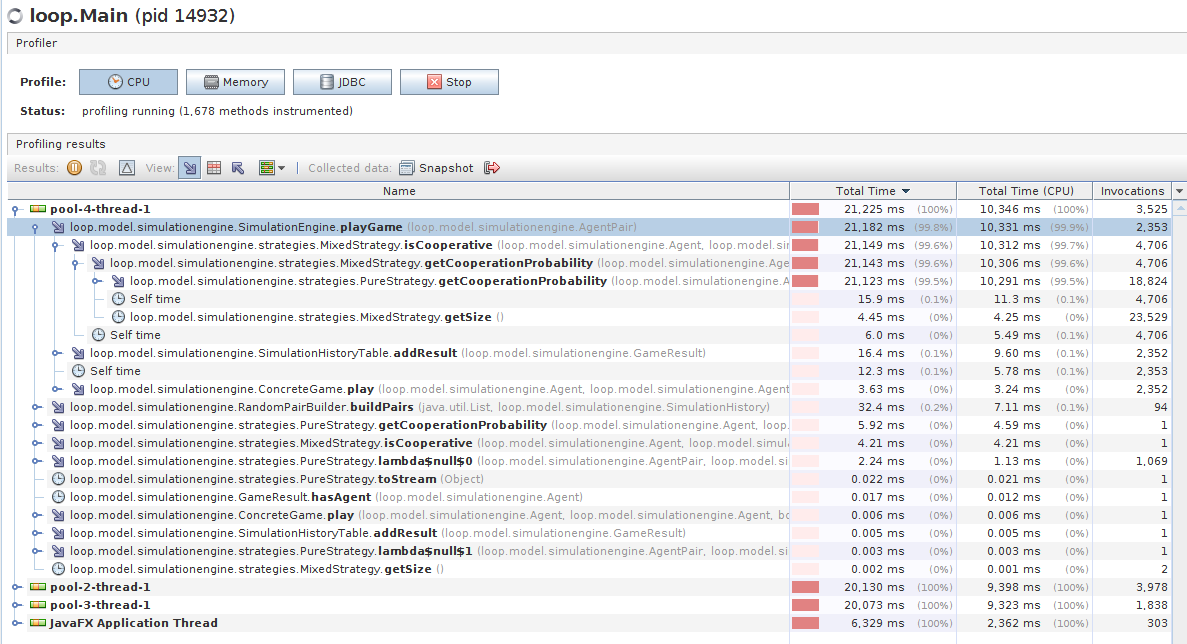
\includegraphics[width=\linewidth]{images/profiler_old.png}
	\caption{Ausgabe des Profilers während einer Simulation}
	\label{profiler_old}
\end{figure}


\section{Änderungen in der Applikation}

\subsection{Erweiterung der Ausgabe}
Es ist nun möglich, die Entwicklung der Strategieverteilung auf der ersten Seite im Ausgabefenster für einzelne Gruppen getrennt zu betrachten. Dazu befindet sich unter dem Diagramm ein Dropdown-Menü, in dem eine Teilmenge aller beteiligten Gruppen ausgewählt werden kann (siehe Abb. \ref{strategydiagram}). Die Strategieverteilung wird dann für die Agenten der ausgewählten Gruppen angezeigt. Insbesondere ergibt sich dasselbe Diagramm wie zuvor, wenn man alle Gruppen auswählt.

\begin{figure}
	\centering
	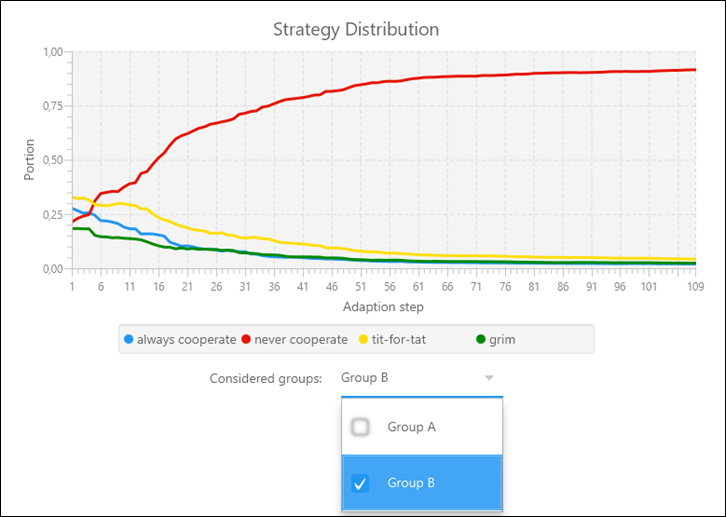
\includegraphics[width=0.8\linewidth]{images/strategydiagram.png}
	\caption{Gruppenauswahl für die Strategieverteilung}
	\label{strategydiagram}
\end{figure}

\subsection{Einstellungsfenster}
Es gibt nun ein Einstellungsfenster, in dem persistente Einstellungen vorgenommen werden können (siehe Abb. \ref{settings_window}):

\begin{itemize}
\item[] \textbf{Benachrichtigungen:} Sind Benachrichtigungen aktiviert, so wird der Nutzer durch eine kurze Nachricht auf abgeschlossene Simulationen hingewiesen (siehe Abb \ref{notification})
\item[] \textbf{Tooltips:} Das Einblenden von Tooltips beim hovern über Knöpfe und andere Elemente kann (de-)aktiviert werden.
\item[] \textbf{Verwendete Threads:} Der Nutzer kann spezifizieren, wie viele der zur Verfügung stehenden (logischen) Prozessorkerne für Simulationen verwendet werde sollen. Damit die GUI auch während dem Ausführen von Simulationen noch flüssig läuft, ist es zu empfehlen, einen Kern freizuhalten.
\item[] \textbf{Ordnerstruktur:} Der Nutzer kann Dateipfade angeben, aus denen (zusätzlich zur vom Programm angelegten Ordnerstruktur) bei Programmstart alle hinterlegten Spiele, Populationen, Gruppen und Strategien geladen werden.
\end{itemize}

\begin{figure}
	\centering
	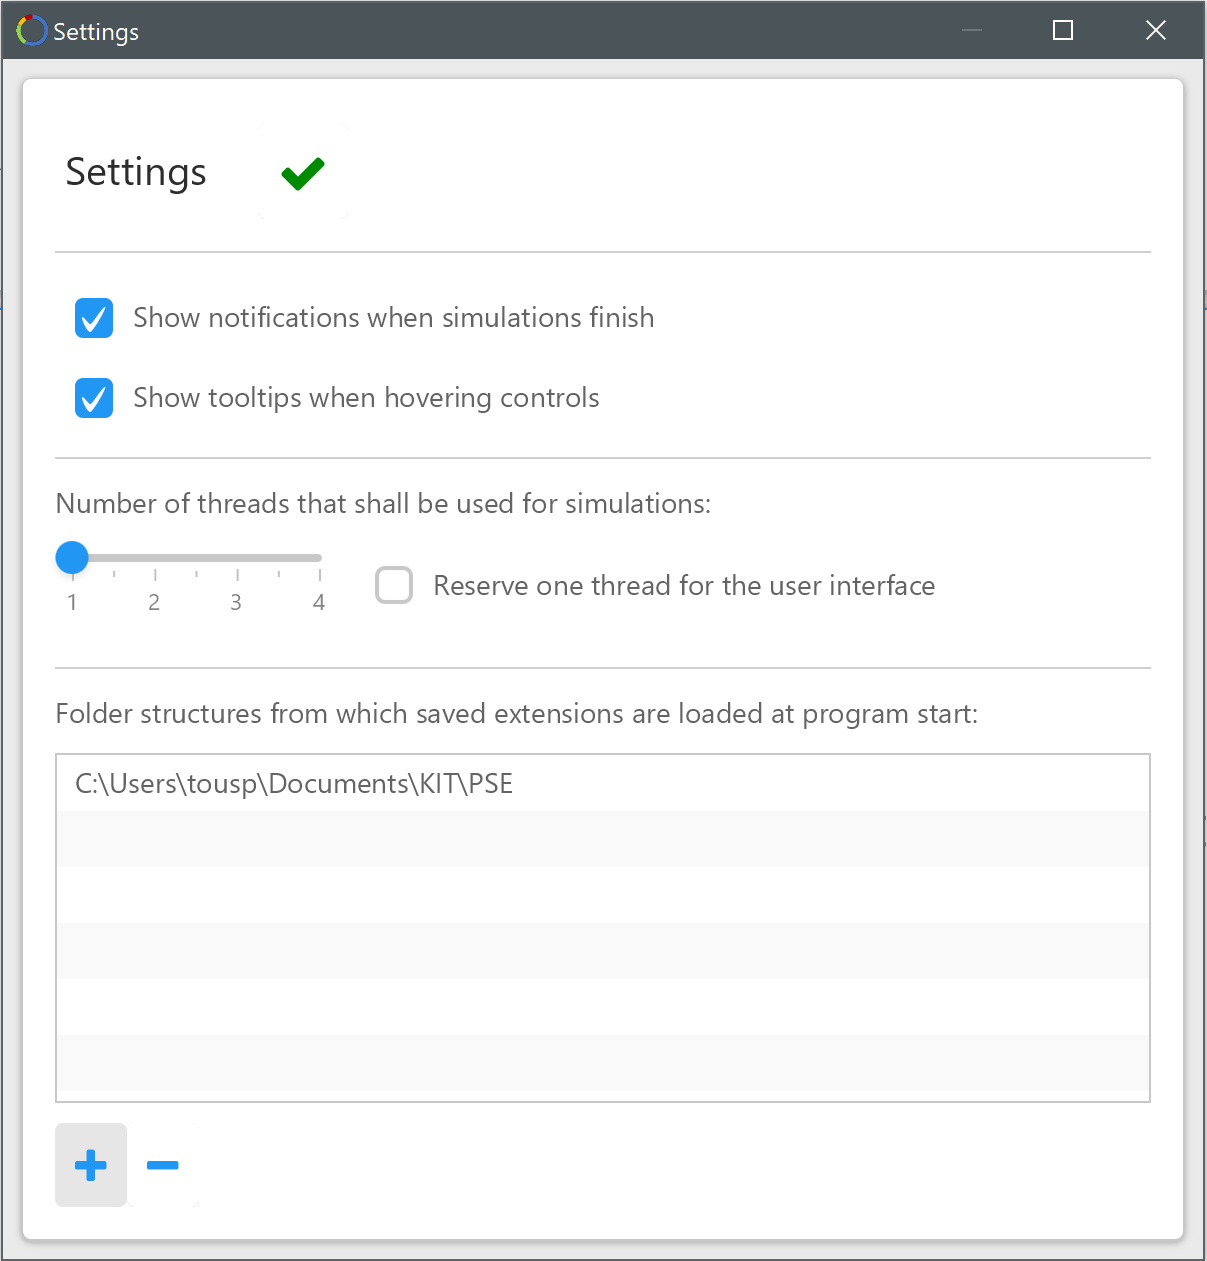
\includegraphics[width=0.8\linewidth]{images/settings_window.png}
	\caption{Einstellungsfenster}
	\label{settings_window}
\end{figure}

\begin{figure}
	\centering
	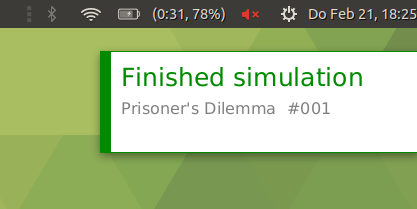
\includegraphics[width=0.4\linewidth]{images/notification.png}
	\caption{Benachrichtigung bei abgeschlossener Simulation.}
	\label{notification}
\end{figure}

\subsection{Entfernen von Simulationen}
Es ist nun möglich, abgeschlossene und abgebrochene Simulationen aus der Ansicht zu entfernen (siehe dazu Abb. \ref{deletesimulation}).

\begin{figure}
	\centering
	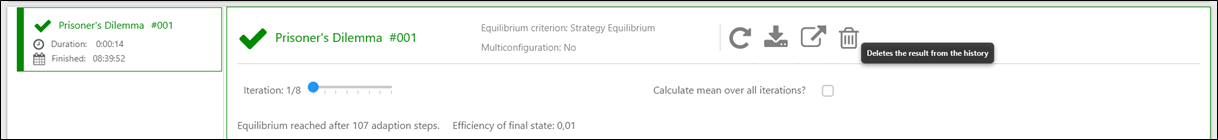
\includegraphics[width=\linewidth]{images/deletesimulation.png}
	\caption{Knopf zum Entfernen einer abgeschlossenen Simulation.}
	\label{deletesimulation}
\end{figure}

\section{Abdeckung der Tests im Pflichtenheft}

Die folgende Tabelle greift die im Pflichtenheft definierten Test auf und gibt an, welche davon getestet wurden. Da es sich fast ausschließlich um GUI-Tests handelt, erfolgte das Testen größtenteils manuell.

Einige Testszenarien wurden an Spezifikationsänderungen angepasst. Etwa hat sich die Struktur des Konfigurationsfensters durch das Einführen von Populationen in der Entwurfsphase geändert.

\begin{table}[h]
	\centering
	\begin{tabular}{@{}ll|c|r@{}}
		\toprule
		&\textbf{Test Nr.} & \textbf{Getestet} &\textbf{Anmerkung} \\ 
		\midrule
		\multicolumn{3}{l|}{\small \textsc{\textbf{T1} Grundeinstellungen}} \\ 
		&T1.1 - T1.4 & \cmark & \\
		&T1.5 & (\xmark) & \makecell{Einstellung wurde mit dem Einführen\\ von Populationen entfernt}\\
		&T1.6 & \cmark & Der Slider wurde durch ein Textfeld ersetzt\\
		&T1.7 & \cmark & \\
		&T1.8 & \cmark & \\
		&T1.9 - T1.10 & (\xmark) & \makecell{Einstellungen wurden mit dem Einführen\\ von Populationen entfernt}\\
		&T1.11 & \cmark & \\ 
		\multicolumn{4}{l}{\small \textsc{\textbf{T2} Simulationen starten und abbrechen, Ergebnisanzeige}}\\ 
		&T2.1 & \cmark & \\
		&T2.2 - T2.3 & \cmark & Der Knopf zum Abbrechen wurde verschoben\\
		&T2.4 - T2.6 & \cmark & \\
		\multicolumn{4}{l}{\small \textsc{\textbf{T3} Konfigurationen und Simulationen speichern und laden}}\\ 	
		&T3.1 - T3.4 & \cmark & \makecell{Konfigurationen werden nun vom Hauptfenster aus\\ geladen und gespeichert}\\
		&T3.5 - T3.9 & \cmark & \\
		\multicolumn{4}{l}{\small \textsc{\textbf{T4} Gruppen- und Segmenteinteilung}}\\ 
		&T4.1 - T4.8 & (\cmark) & \makecell{Die Gruppenerstellung wurde mit dem Einführen von\\ Populationen überarbeitet und entsprechend getestet} \\
		\multicolumn{3}{l|}{\small \textsc{\textbf{T5} Stufenspiel erstellen}}\\ 
		&T5.1 - T5.2 & \cmark & \\
		\multicolumn{4}{l}{\small \textsc{\textbf{T6} Festlegung des Algorithmus zur Paarbildung}}\\ 
		&T6.1 - T6.2 & \cmark & \\
		\multicolumn{4}{l}{\small \textsc{\textbf{T7} Festlegung der Erfolgsquantifizierung}}\\ 
		&T7.1 - T7.3 & \cmark & \\
		\multicolumn{4}{l}{\small \textsc{\textbf{T8} Festlegung des Adaptionsmechanismus}}\\ 
		&T8.1 - T8.3 & \cmark & \\
		\multicolumn{4}{l}{\small \textsc{\textbf{T9} Gleichgewichtskriterium und Schranke für Adaptionsschritte festlegen}}\\ 
		&T9.1 - T9.4 & \cmark & \\
		\multicolumn{3}{l|}{\small \textsc{\textbf{T10} Multikonfiguration}}\\ 
		&T10.1, T10.3 & \cmark & \makecell{Die Einstellung des Multi-Parameters erfolgt nun\\ über ein dediziertes Dropdown-Menü}\\
		&T10.2, T10.4 - T10.6 & \cmark & \\
		\multicolumn{3}{l|}{\small \textsc{\textbf{T11} Strategie erstellen}}\\
		&T11.1 - T11.3 & \cmark & \\
		\multicolumn{3}{l|}{\small \textsc{\textbf{T12} Fehlerbehandlung}}\\ 
		&T12.1, T12.3 - T12.7 & (\xmark) & \makecell{Einstellungen wurden mit dem Einführen\\ von Populationen entfernt}\\
		&T12.2 & (\cmark) & \makecell{Statt einer Autokorrektur wird eine fehlerhafte\\ Eingabe entsprechend markiert}\\
		\bottomrule
	\end{tabular}
	\caption{Übersicht zur Abdeckung der Test aus dem Pflichtenheft}
\end{table}

\section{Statistiken}

Unser Programm wurde in 41 Testklassen und 186 Tests in insgesamt 2728 Zeilen Testcode getestet.

Betrachtet man die mit JUnit sinnvoll zu testenden Pakete, so wird eine Testabdeckung von 96,7\% erreicht. Das entspricht 86,7\% des Models und 30,2\% des gesamten Quellcodes, wo auch Controller und View mit inbegriffen sind.

\chapter{Fehlerprotokoll}

\section{Fehler mit Ursprung im Model}

\textbf{Die Syntax von selbsterstellten Strategien wurde nicht korrekt geprüft.} \newline
\textbf{Grund: } Der Algorithmus zum Erkennen von fehlerhaften Teilbäumen des Syntaxbaumes war nicht korrekt implementiert. Der kleinste fehlerhafte Teilbau, wird nicht richtig erkannt. Insbesondere konnte manchen Fällen eine Endlosschleife auftreten.
\newline
\textbf{Behebung: } Der entsprechende Algorithmus wurde korrigiert.

\textbf{Strategien, bei denen sich der Agent darauf bezieht, ob Agenten aus seiner Gruppe gegen diesen bestimmten Gegner kooperiert haben, schlugen Fehl.} 
\newline
\textbf{Grund: } Bei der Implementierung der jeweiligen Strategien, wurde auf falsche Agenten zugegriffen, sodass auch Spiele zwischen Agenten berücksichtigt wurden, die nicht hätten dürfen.
\newline
\textbf{Behebung: } Größere Umstrukturierungen bei der Implementierung von den jeweiligen Strategien. 

\textbf{Selbsterstellte Strategien konnten nicht abgespeichert werden, wenn bestimmte Prädikate verwendet wurden.} 
\newline
\textbf{Grund: } Manche der Prädikate, die zum Erstelle eigener Strategien verwendet werden können waren nicht serialisierbar, da bei der Implementierung Java 8 Lambda-Ausdrücke verwendet wurden, die standardmäßig nicht serialisierbar sind.
\newline
\textbf{Behebung: } Die Lambda-Ausdrücke wurden durch serialisierbare Lambda-Ausdrücke ersetzt.

\textbf{Simulationen mit einer \enquote{Multiconfiguration} erzeugten teilweise falsche Ergebnisse (bspw. wurden Gleichgewichte nicht erkannt).} 
\newline
\textbf{Grund: } Beim Erstellen der einzelnen Konfigurationen aus einer \texttt{UserConfiguration} wurden die gleichen Instanzen der verwendeten Algorithmen für alle elementaren Konfigurationen verwendet. Dies führte bei der Ausführung einer Simulation zu Wettlaufbedingungen zwischen verschiedenen threads.
\newline
\textbf{Behebung: } Alle elementaren Konfigurationen erhalten eine eigene Instanz der verwendeten Algorithmen.

\textbf{Simulationen mit einer Simulationsdauer im Millisekundenbereich erzeugten teilweise Fehler} 
\newline
\textbf{Grund: } Solche kurzen Simulationen wurden manchmal bereits abgeschlossen, bevor im Conroller die nötigen Behandlungsroutinen registriert wurden. Das führte dazu, dass das Beenden einer Simulation nicht erfasst wurde, oder  \texttt{ConcurrencyException}s geworfen wurden.
\newline
\textbf{Behebung: } Die Klasse \texttt{SimulationResult} wurde um verschiedene Synchronisationsmechanismen erweitert.



\section{Fehler mit Ursprung in der Benutzeroberfläche}

\textbf{Wurden im Fenster zum Erstellen eigener Strategien Prädikate auf Wurzeleben des Syntaxbaums gelöscht, blieb die Benutzeroberfläche unverändert. } 
\newline
\textbf{Grund: } Die internen Datenstrukturen wurden  korrekt aktualisiert, jedoch nicht die Benutzeroberfläche
\newline
\textbf{Behebung: } Die Benutzeroberfläche wird korrekt aktualisiert, indem der entsprechene Methodenaufruf ergänzt wurde.

\end{document}
